\documentclass[10pt]{standalone}
\usepackage[utf8]{inputenc}
\usepackage{pgf,tikz }
%\pgfplotsset{compat=1.15}
\usepackage{mathrsfs}
\usetikzlibrary{arrows}
\pagestyle{empty}
\begin{document}

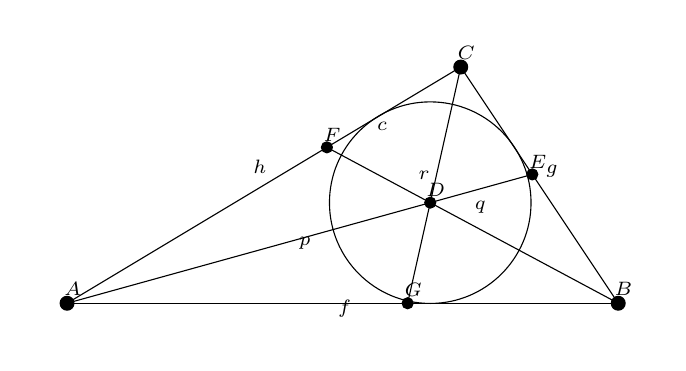
\begin{tikzpicture}[line cap=round,line join=round,>=triangle 45,x=1.0cm,y=1.0cm]

\clip(-0.5,-0.5) rectangle (7.5,3.5);
\draw  (0.,0.)-- (7.,0.);
\draw  (7.,0.)-- (5.,3.);
\draw  (5.,3.)-- (0.,0.);
\draw  (4.612700309690656,1.2776440208969848) circle (1.28cm);
\draw  (0.,0.)-- (5.908888435188947,1.6366673472165794);
\draw  (7.,0.)-- (3.3001584821877885,1.980095089312673);
\draw  (5.,3.)-- (4.3254013194571215,0.);
\begin{scriptsize}
\draw [fill=black] (0.,0.) circle (2.5pt);
\draw (0.07298849002481059,0.18534122375859213) node {$A$};
\draw [fill=black] (7.,0.) circle (2.5pt);
\draw (7.067235042745172,0.18534122375859213) node {$B$};
\draw [fill=black] (5.,3.) circle (2.5pt);
\draw (5.068878884825069,3.182875460638748) node {$C$};
\draw (3.525593931183801,-0.07187293518161927) node {$f$};
\draw (6.157092634187501,1.6791619160652043) node {$g$};
\draw (2.4472730340882998,1.7286261773998604) node {$h$};
\draw [fill=black] (4.612700309690656,1.2776440208969848) circle (2.0pt);
\draw (4.683057646414752,1.4417334616588553) node {$D$};
\draw (4.000450839996499,2.2529473475472144) node {$c$};
\draw [fill=black] (5.908888435188947,1.6366673472165794) circle (2.0pt);
\draw (5.97902129338274,1.7978761432683787) node {$E$};
\draw [fill=black] (3.3001584821877885,1.980095089312673) circle (2.0pt);
\draw (3.3673082949129016,2.144125972610971) node {$F$};
\draw [fill=black] (4.3254013194571215,0.) circle (2.0pt);
\draw (4.396164930673747,0.16555551922472972) node {$G$};
\draw (3.0210584655703094,0.7591266552406022) node {$p$};
\draw (5.24695022562983,1.2141978595194376) node {$q$};
\draw (4.534664862410784,1.6198048024636171) node {$r$};
\end{scriptsize}

\end{tikzpicture}
\end{document}